\section{Neural Networks}

\subsection{Deep Learning}

The concepts of deep learning studied in this section is going to be based on the work of \citet{goodfellow2016} and the documentation of PyTorch\footnote{\url{https://pytorch.org/docs/stable/index.html}} and MATLAB\footnote{\url{https://www.mathworks.com/help/matlab/}}.

There are several definitions of \gls*{ai} \citep{winston1992}, but the  computer scientist \citet{mccarthy2007} defines it as ``the science and engineering of making intelligent machines, especially intelligent computer programs.''.
He also states that ``it is related to the similar task of using computers to understand human intelligence, but AI does not have to confine itself to methods that are biologically observable.''.

The big area of study is the \gls*{ai} and it includes several branches like fuzzy logics, robotics, machine learning and so on. 
The later one, in turn, is another field with also some branches and one of them is the deep learning.
This can be represented in a Venn diagram, as the \cref{fig:venn_dl} shows.
However, all the three terms can be interchangeable in the major context.

\begin{figure}
    \centering
    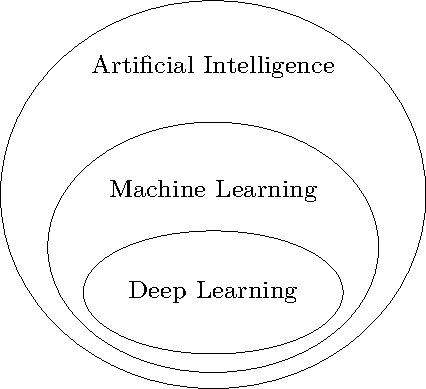
\includegraphics{figures/2methodology/nn/venn_dl.pdf}
    \caption{Subareas of Artificial Intelligence}
    \label{fig:venn_dl}
\end{figure}

The deep learning history goes back to the 1940s and it had several names over the years. It was called by \emph{cybernetics} (1940s--1960s), \emph{connectionism} (1980s--1990s), and from 2006 until now is known as \emph{deep learning}.
The \gls*{dl} models were engineered systems inspired by the biological brain and they were denominated \gls*{ann}.
One of the motivations of the neural perspective was to understand that the brain provides a proof by example that intelligent behavior is possible and try to reverse engineer the computation principals behind the brain, duplicating its functionality.

\gls*{dl} today goes beyond the neuroscientist perspective and it is more of general principle of learning multiple levels of composition.

\subsection{Multilayer Perceptron}

\subsubsection*{Perceptron}

A perceptron is a supervised learning algorithm that provides binary classifiers. It is the simplest kind of \gls*{ann}, but the complex ones are based on it and it serves to solve many problems yet.

\begin{figure}
    \centering
    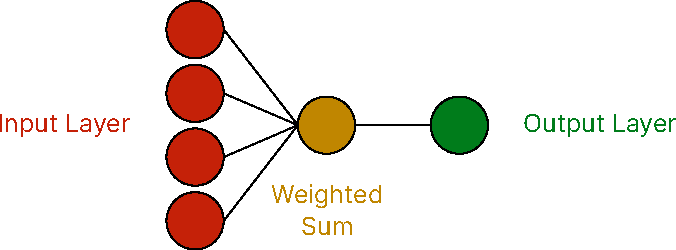
\includegraphics{figures/2methodology/nn/perceptron.pdf}
    \caption[Perceptron Scheme]{Perceptron Scheme. It is a simple machine learning algorithm that provides a binary output. It resembles a human neuron: input layer data is equivalent to the dendrites; hidden layers are the equivalent of the axons; and the output layer are the equivalent of the nerve ending.}
    \label{fig:perceptron}
\end{figure}

The principle is quite simple, from the input data \(\mathbf{x}\) and initial random weights \(\mathbf{w}\), it returns the weighted sum \(f(\mathbf{x},\mathbf{w})\). This is graphically represented in the~\cref{fig:perceptron}.
%
\begin{equation}\label{eq:perceptron_weighted_sum}
    f(\mathbf{x},\mathbf{w}) = \sum_{i=1}^n x_iw_i =  x_1w_1 + x_2w_2 + \cdots + x_nw_n
\end{equation}
%
where \(\mathbf{x}\) is a vector containing the input data and \(\mathbf{w}\) is a vector containing the weights, both with \(n\) elements.

It splits the data with a straight line classifying them in two groups and that is the reason it is a binary classifier.

\begin{figure}
    \centering
    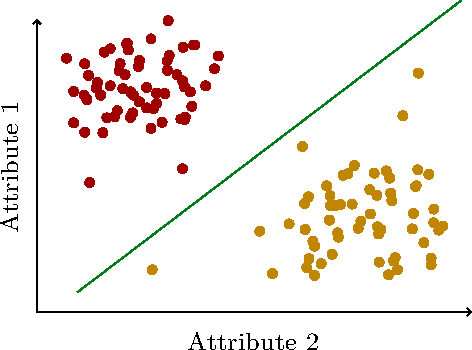
\includegraphics{figures/2methodology/nn/perceptron_charge.pdf}
    \caption[Perceptron Behavior]{Perceptron Behavior. It is a binary classifier.}
\end{figure}

Surely, for the first iteration, the output should not be the best one and the procedure must begin from the start, but now with the new values obtained. Then, for each iteration it tends to get a better and learn to label each data received.
 
A \gls*{mlp}, also known as \emph{deep network}, is the essence of \gls*{dl}. Basically, it is a mathematical function, formed by composing many simpler functions, mapping some set of input values to output values.
%
\begin{figure}
    \centering
    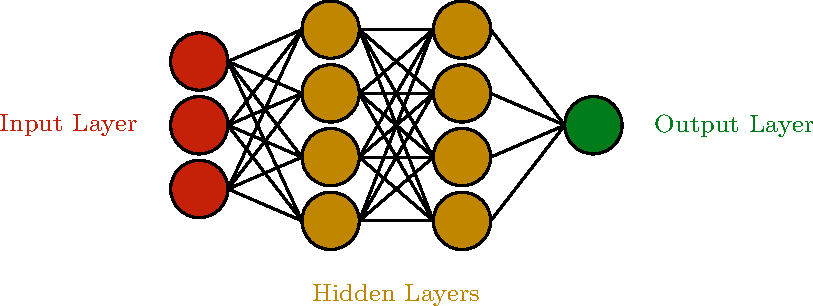
\includegraphics{figures/2methodology/nn/mlp.pdf}
    \caption[Multilayer Perceptron Scheme]{Multilayer Perceptron Scheme. The figure show two hidden layers, totalizing eight neurons. A \gls*{mlp} accepts multiple hidden layers and neurons. It can also have several outputs.}
\end{figure}